\documentclass[../../../../main.tex]{subfiles}
\begin{document}

図のように，三角形 $ABC$ の内接円よりはじめて，
次々と前の円と外接し，
かつ三角形の2辺に接する円を3つの頂点に向かってえがいていく。
このとき，三角形内にあるすべての円の面積の総和を，
内接円の半径 $r$ と3つの内角 $A$，$B$，$C$ で表わせ。
とくに，1辺 $a$ の正三角形の場合に，この総和はいくらか。

\begin{figure}[htbp]
  \centering
  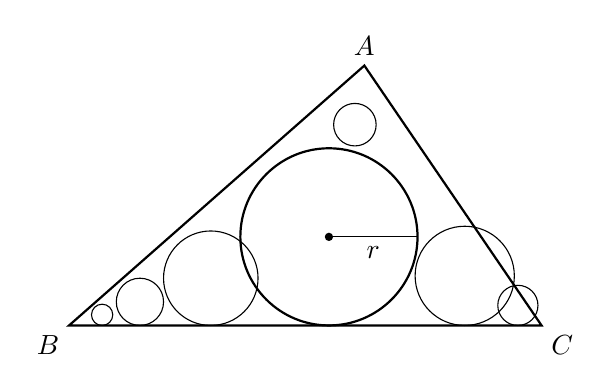
\begin{tikzpicture}[scale=1.5]
    \coordinate (B) at (0,0);
    \coordinate (C) at (4,0);
    \coordinate (A) at (2.5,2.2);

    \draw[thick] (A) -- (B) -- (C) -- cycle;
    \node[above] at (A) {$A$};
    \node[below left] at (B) {$B$};
    \node[below right] at (C) {$C$};

    % 主内接円
    \coordinate (I) at (2.2, 0.75);
    \def\r{0.75}
    \draw[thick] (I) circle (\r);
    \fill (I) circle (1pt);
    \draw (I) -- node[below] {$r$} +(0:\r);

    % 頂点A方向の小円
    \draw (2.42, 1.7) circle (0.18);

    % 頂点B方向の小円列
    \draw (1.2, 0.4) circle (0.4);
    \draw (0.6, 0.2) circle (0.2);
    \draw (0.28, 0.09) circle (0.09);

    % 頂点C方向の小円列
    \draw (3.35, 0.42) circle (0.42);
    \draw (3.8, 0.17) circle (0.17);
  \end{tikzpicture}
\end{figure}

\end{document}
